\begin{figure}[htbp]
\centering
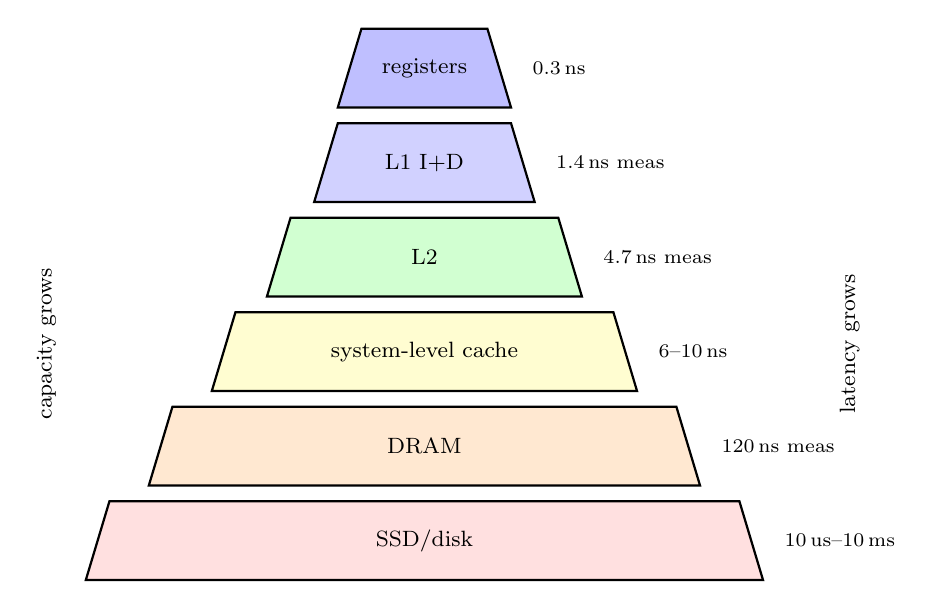
\begin{tikzpicture}[font=\footnotesize, x=1cm, y=1cm]
  \foreach \y/\w/\lbl/\lat/\fill in
    {5.6/2.2/{registers}/{0.3\,ns}/blue!25,
     4.4/2.8/{L1 I+D}/{1.4\,ns meas}/blue!18,
     3.2/4.0/{L2}/{4.7\,ns meas}/green!18,
     2.0/5.4/{system-level cache}/{6--10\,ns}/yellow!18,
     0.8/7.0/{DRAM}/{120\,ns meas}/orange!18,
     -0.4/8.6/{SSD/disk}/{10\,us--10\,ms}/red!12} {
    \draw[thick, fill=\fill] ({-\w/2},\y) -- ({\w/2},\y) --
        ({\w/2-0.3},\y+1.0) -- ({-\w/2+0.3},\y+1.0) -- cycle;
    \node at (0,\y+0.5) {\lbl};
    \node[anchor=west, font=\scriptsize] at ({\w/2+0.15},\y+0.5) {\lat};
  }
  \node[rotate=90, anchor=center] at (-4.8,2.6) {capacity grows};
  \node[rotate=90, anchor=center] at (5.4,2.6) {latency grows};
\end{tikzpicture}
\caption{The hierarchy pyramid with \emph{measured} numbers from
this chapter's runs (Apple Silicon arm64): roughly
0.3\,ns$\to$1.4\,ns$\to$5\,ns$\to$10\,ns$\to$120\,ns from register
to DRAM --- four orders of magnitude before storage even enters.}
\label{fig:pyramid09}
\end{figure}
